\documentclass[pdf, color,12pt]{CITnote}
%optional [color] for a color logo .

\usepackage[export]{adjustbox}
\usepackage[utf8]{inputenc}
\usepackage[T1]{fontenc}
\usepackage{graphicx}
\usepackage{titlepic}
\usepackage{mathtools}
\usepackage{soul}
\usepackage{amsmath}
\usepackage{amssymb}
\usepackage{amsthm}
\usepackage{tabu}
\usepackage{float}
%\usepackage[demo]{graphicx}
\usepackage{subfig}
\usepackage{ulem}
\usepackage{amsfonts}
\usepackage{accents}
%\usepackage{subcaption}
\usepackage{multicol}
\usepackage{hyperref}
\usepackage{enumitem}
\usepackage{listings}
\usepackage{mathtools}
\usepackage{fixmath}
\usepackage[justification=centering]{caption}

\usepackage[font=small,labelfont=bf, skip=10pt]{caption}


\usepackage{makecell}

\renewcommand\theadalign{bc}
\renewcommand\theadfont{\bfseries}
\renewcommand\theadgape{\Gape[4pt]}
\renewcommand\cellgape{\Gape[4pt]}

\usepackage[margin=30mm]{geometry}
\usepackage{changepage}

\author{\begin{LARGE} Garbi Luca \end{LARGE}}
%\refnum{S2....}
\shorttitle{}
\title{\begin{LARGE}- Winter School on Physics of the Cell -
\\ Modelling phototransduction and other biochemical networks\end{LARGE}}
\date{\begin{Large} \today \end{Large}}
\issue{1}



\newcommand{\tcr}{\textcolor{red}}
\newcommand{\tcb}{\textcolo r{blue}}
\newcommand{\tcm}{\textcolor{magenta}}
\newcommand{\tcg}{\textcolor{green}}
\newcommand{\tcp}{\textcolor{purple}}

\begin{document}

\maketitle

%\section{la}

	%\addtolength{\oddsidemargin}{.875in}
	%\addtolength{\evensidemargin}{.875in}
	
\begin{adjustwidth*}{0.4cm}{0.4cm}
\begin{center}
\section*{\large Introduction}
\end{center}

{\bf{This report is based on the hands-on session, given at the University of Trento by Prof. Daniele Dell'Orco, on January 29$^{th}$, 2020, in the context of the Winter School on Physics of the Cell. The objective of this write-up is on one hand to briefly synthesize the lecture on the modelling of dynamic biophysical systems, on the other hand to implement a simplified model of phototransduction via the ODE-based version of \textsc{IQMtools}, i.e.$ $ a \textsc{MATLAB} toolbox used in class for the implementation of a different biophysical system.
}}\\
\end{adjustwidth*}



\section{\large Modelling of biophysical systems}
In order to model a network structure in a formal way we need at first to define the reactants, the products and the modifiers of the structure. While we are doing that, we obviously also need to keep in mind that, for a particular biophysical system, in general there is more than one reaction. So the reactant of one of these could be the product of another one. To address this fact we use a single vector $\textbf{P}$ to identify the concentration of the $N$ products, reactants and eventually modifiers. Moreover if we know the rate at which every reaction occurs we can stuck them in an array $\textbf{R}=(R_1, R_2, ..., R_n)^T$, where $R_i$ is the rate at of the i-th reaction. Now it is simple to link these two vectors since we know the stoichiometric information of the reactions, it is important though to bear in mind that by doing that we are assuming that our system is described by a static model. We use the stoichiometric matrix $\mathbold{\chi} \in \mathcal{M}_{Nn}(\mathbb{R})$, which is composed of the coefficients of the reactants or products (in columns) for every reaction (in rows). Now we can write all the dynamic of our biophysical system in a formal way by the relation $\frac{d}{dt}\textbf{P}=\mathbold{\chi}\textbf{R}$. Since $\textbf{R}$ isn't a constant, but a function of $\textbf{P}$ what we have is an ordinary differential equation. To solve these type of ODEs we can use numerical integration methods but the problem now is to determine the mathematical expressions for the reactions rate.
\newline
In order to do that we use the \textit{law of mass action}, and here we are making a second assumption. This law says that the rates of the reactions are directly proportional to the product of the activities or concentrations of the reactants, but it holds only in the case of dynamic equilibrium. The statement is true, strictly speaking, only for elementary reactions made of a single mechanistic step. Hence we are assuming that every reaction we are modelling is an elementary reaction, we are basically neglecting intermediate steps. That is not always true, in fact macromolecular interactions depend on several factors beyond concentration, such as temperature, the presence of a solvent, pressure or stirring.
\\ Given $A_i, B_i, C_i$ and $D_i$ reactants and products of the i-th reaction
$$ aA_i+bB_i\longleftrightarrow cC_i+dD_i
$$
with $a,b,c,d$ stoichiometric coefficients, than the total rate of the $R_i$ can be written as
$$ R_i = k_1[A_i]^a[B_i]^b-k_2[C_i]^c[D_i]^d
$$
in this case $k_1$ and $k_2$ are the constants for the forward and backward part of the reaction.
\\ In the case instead of an enzymatic reaction, if we consider an enzyme E binding to a substrate S, to form a complex ES which releases the product P, than we can write
$$E+S\xleftrightarrow[\ \ k_b \ \ ]{\ \ k_f \ \ } ES \xrightarrow{\ k_{cat} \ } E+P
$$
introducing the forward, backward and catalytic rate constants.
Now we exploit the Michaelis-Menten equation - which holds in the same assumption domain discussed above - in order to write the reaction rate as
$$R_e=\frac{V_{max}\cdot [S]}{k_d+[S]}
$$
where $k_d=(k_{cat}+k_b)/k_f$ is again an unvarying real number, namely a constant of dissociation, and $V_{max}\doteq k_{cat}\ [E]_{tot}$.
\\ Now the problem reduces to the determination of all the $k_i$ constants for our reactions.
The parameters are not entirely inferred experimentally, but the estimation process consist of a feedback loop that exploits both experimental and simulated data. The workflow for the parameter values determination can be outlined as follows
\begin{figure}[ht!]
\centering
\centerline{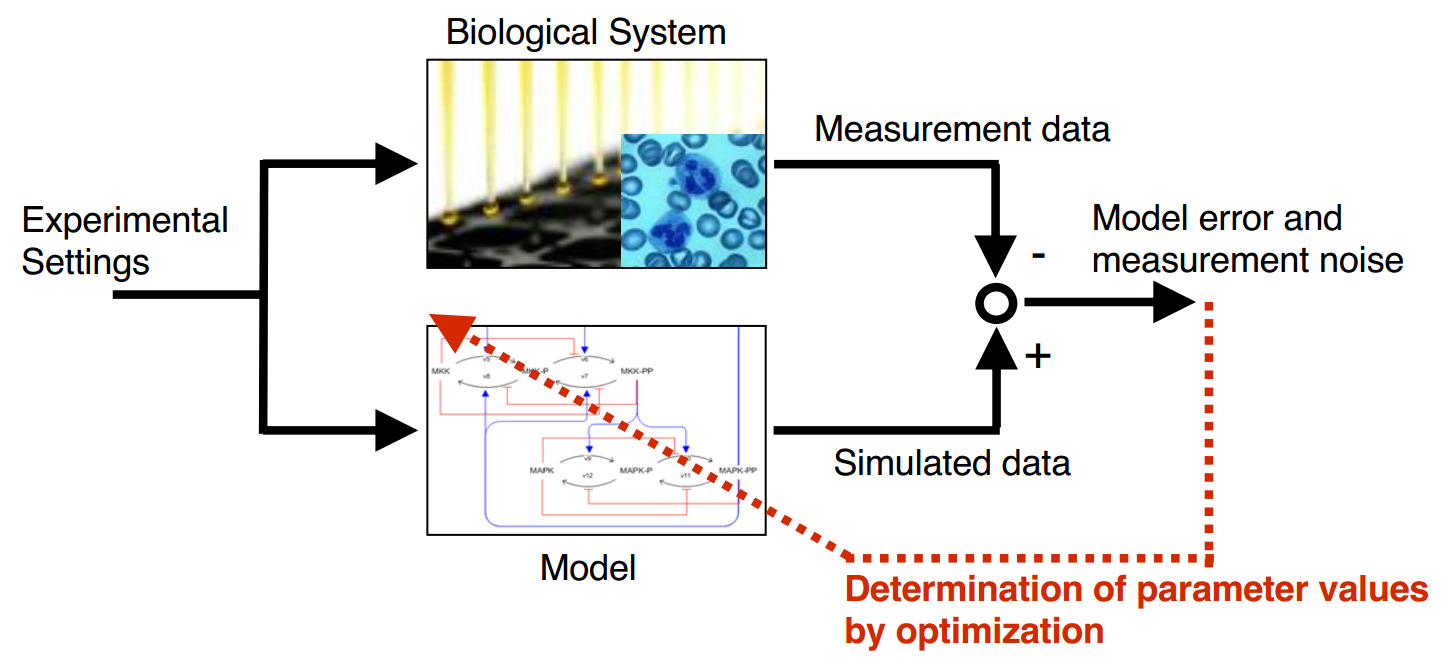
\includegraphics[scale=0.25]{WS1.png}}
\end{figure}


\section{{\large \textsc{IQMtools} implementation of a phototransduction model}}

The phototransduction model we want to implement is inspired by the work of \textit{Felber et al.}, taken by the \textit{Biophysical Journal} (\textbf{71}), 1996, 3051-3063.
\\ This model exploits a mesoscopic approach that neglects any detail of intra- or intermolecular reaction: basically protein-protein
interaction is approximated by a single step that simultaneously include the
encounter and reaction of two proteins. Furthermore, it is assumed
that any reaction or diffusion step is independent of the
history of the system. 
This will allow us to use an ODE solver for the equations that rule the systems as illustrated in the first section.
\\ The system we are studying is an example of a G-protein cascade of reactions happening on rod disc membranes. It consists of the photoreceptor rhodopsin ($R$), the G-protein transducin ($G_t$), and a
phosphodiesterase (PDE) effector, which hydrolyzes cytosolic cyclic guanosine monophosphate (cGMP). This nucletide is a common regulator of ion channel conductance, in fact the sodium ion channels in the eye photoreceptors are cGMP-gated, so degradation of cGMP causes sodium channels to close. When this happens there is an hyperpolarization of the photoreceptor's plasma membrane that leads to visual information being sent to the brain.
\\
The first single-step reaction, as labelled in Fig.$ $ \ref{fig: one}, consist of the multistep transition of rhodopsin into an active state $R^*$.
\begin{figure}[ht!]
\centering
\centerline{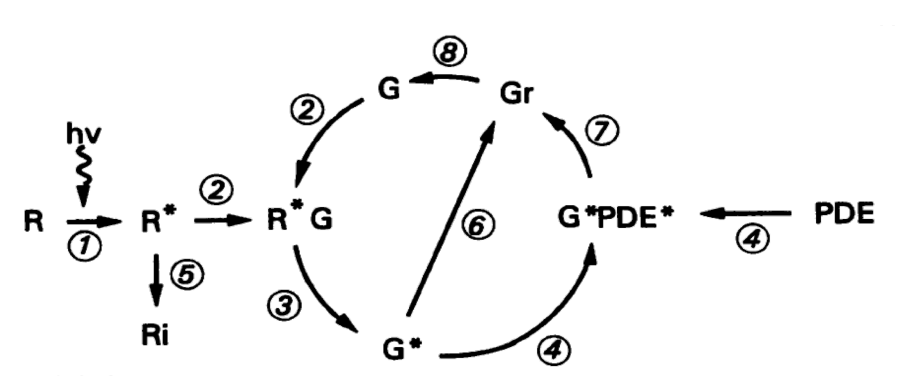
\includegraphics[scale=0.4]{WS2.png}}
\caption{\small{ Model of the Transducin GTPase cycle, taken from \textit{Felber et al.}, \textit{Biophysical Journal} (\textbf{71}), 1996, 3051-3063. }}
\label{fig: one}
\end{figure}
This conversion takes place within milliseconds after the absorption of a single photon. In the second step there is the coupling of the active rhodopsin to the G-protein transducin ($R^*+G_t\rightarrow R^*G_t$). This reaction is followed immediately after by the dissociation of $R^*G_t$ leaving free active rhodopsin and GTP-bound $G^*$ (reaction 3). The $G^*$ molecule now bind to the PDE thus forming the cGMP-hydrolyzing effector enzyme ($G^*+$PDE$\rightarrow G^*$PDE$^*$). With this $4^{th}$ reaction ends also the activation step; during the deactivation one, the active rhodopsin make a transition into inactive ($R_i$) and the $G^*$ goes into a refractory state $G_r$ (reactions 5 and 6). Also the dissociation of $G^*$PDE$^*$ creates some $G_r$ along with inactive phosphodiesterase effector.
In the last step (reaction 8) there is the recycling of the G-protein from the refractory state to the holoprotein $G_t$ that is again ready for interaction with the receptor.
\\ One particular that is important to bear in mind is that photoactivated rhodopsin (R*) molecules catalytically activate many copies of the G-protein (which in turn binds and activates the effector). Moreover the deactivation of $R^*$ may comprise different reaction states, namely, binding and activation of rhodopsin kinase, phosphorylation of $R^*$, and binding of arrestin. Therefore our model of a
first-order decay of $R^*$ to $R_i$ implies a strong assumption on the velocity - that is supposed to be fast relatively to the other processes - of the intermediate steps required for the deactivation.
\\ The \textsc{IQMtools} code used for the simulation can be found in the Appendix. With obvious notation, in the \textit{MODEL PARAMETERS} section, one can found the constants for the reaction rates: the values used for this parameters were taken from the article by \textit{Felber et al.} mentioned above.
\\ In Fig.$ $ \ref{fig: two} is shown the result of the simulation, carried on for 4 seconds, in the case of a single rhodopsin activation by a photon.
\begin{figure}[ht!]
\centering
\centerline{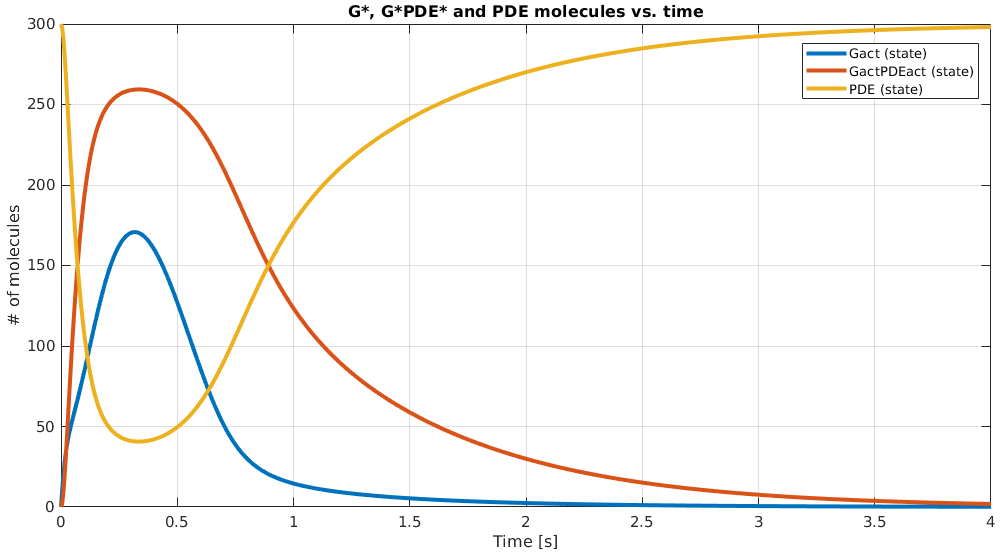
\includegraphics[scale=0.375]{prima.png}}
\caption{\small{Number of $G^*$, $G^*$PDE$^*$ and PDE molecules as a function of time.}}
\label{fig: two}
\end{figure}
We can see a similar kinetics for $G^*$ and $G^*$PDE$^*$ since they both start from zero and have a maximum at about 0.32 s. As we expect, initially the number of $G^*$ molecules is greater than the one of $G^*$PDE$^*$, but after less than 50 ms the amount $G^*$PDE$^*$ created overcome the $G^*$ available. Since the latter molecule is needed for the formation of the former one, is natural to have again a 50 ms delay between the two maxima.  
\\ The simulation with the same initial parameters, except for the number of rhodopsin photoactivations (that in this case is 2), is shown in Fig.$ $ \ref{fig: three}.

\begin{figure}[ht!]
\centering
\centerline{$\  $ 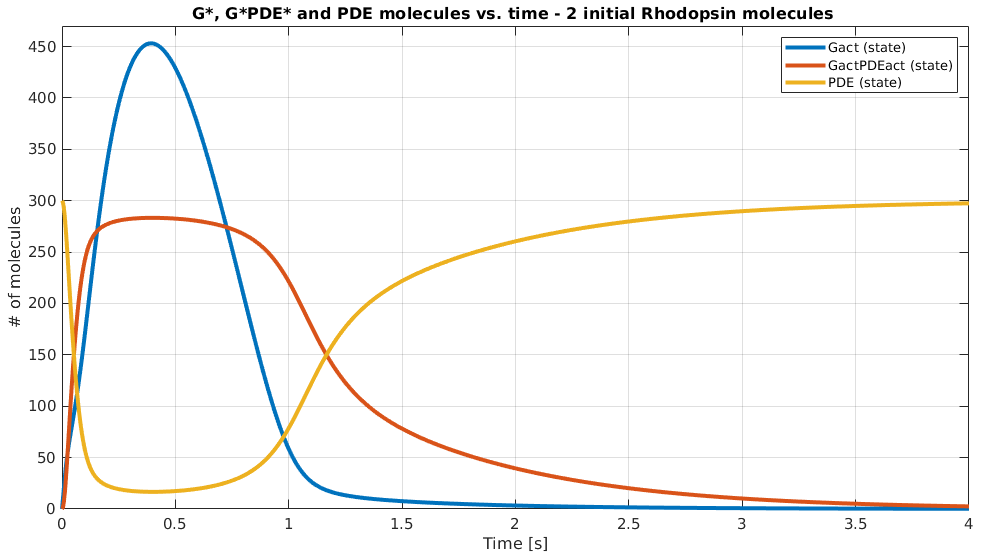
\includegraphics[scale=0.38]{seconda.png}}
\caption{\small{Number of $G^*$, $G^*$PDE$^*$ and PDE molecules as a function of time for 2 photoactivations of rhodopsin.}}
\label{fig: three}
\end{figure}
Of course we notice a substantial increase with regard both to the $G^*$ and $G^*$PDE$^*$ molecules. The interesting fact is that despite the abundance of active G-protein (that more than doubled from the previous case), the cGMP-hydrolyzing effector enzyme can not be formed since there is an upper bound coming from the number of the PDE molecules. What happens instead is that the number of molecules of the enzyme is sensibly high for a longer period of time (basically there is a flattening of the maximum), thus allowing the degradation of cGMP not more intensely but more lasting in time.
\\ As for the number of PDE molecules we can see that in both cases the time that correspond to the minimum is the same of the one that correspond to the maximum of $G^*$PDE$^*$, this happens since in our model the phosphodiesterase is supposed to have interactions only with the $G^*$PDE$^*$ contributing to its formation.

\newpage
\section{{\large Appendix}}
Code used for the ODE-based version of \textsc{IQMtools}:
\\
\\
\begin{lstlisting}
********** MODEL NAME
Hofmann model for phototransduction

********** MODEL NOTES
Biophysical Journal Volume 71, 1996, 3051-3063

********** MODEL STATES
d/dt(G) = -R2+R8 
d/dt(Gact) = +R3-R4-R6 
d/dt(GactPDEact) = +R4-R7 
d/dt(Gr) = +R6+R7-R8 
d/dt(PDE) = -R4+R7 
d/dt(R) = -R1 
d/dt(Ract) = +R1-R2+R3-R5 
d/dt(RactG) = +R2-R3 
d/dt(Ri) = +R5 

G(0) = 3000
Gact(0) = 0
GactPDEact(0) = 0
Gr(0) = 0
PDE(0) = 300
R(0) = 1
Ract(0) = 1
RactG(0) = 0
Ri(0) = 0

********** MODEL PARAMETERS
k1 = 100 
k2 = 1 
k3 = 7000 
k4 = 0.3 
k5 = 2 
k6 = 0.05 
k7 = 8 
k8 = 2 


********** MODEL VARIABLES


********** MODEL REACTIONS
R1 = k1*R
R2 = k2*Ract*G
R3 = k3*RactG
R4 = k4*Gact*PDE
R5 = k5*Ract
R6 = k6*Gact
R7 = k7*GactPDEact
R8 = k8*Gr


********** MODEL FUNCTIONS

\end{lstlisting}

\end{document} 






